\documentclass[12pt, a4paper]{report}
\usepackage[utf8]{inputenc}
\usepackage[top=1.65in, bottom=1.65in, left=1.65in, right=1.65in]{geometry}
\usepackage{listings} %code
\usepackage{graphicx} %images
\usepackage{tikz} %graphs
\usepackage{pgfplots} %plots
\usepackage[mathscr]{eucal} %letter maths

% \usepackage{fancyhdr}
% \usepackage{rotating}
% \usepackage[graphicx]{realboxes}
% \renewcommand{\vec}{\bm}
% \usepackage{dsfont}
% \usepackage{xcolor}
% \usepackage{sectsty}
% \usepackage{amsthm}
% \usepackage{amsmath}
% \usepackage{amsfonts}
% \usepackage{amssymb}
% \usepackage{pgfgantt}
% \usepackage[backend=biber]{biblatex}
% \addbibresource{report.bib}


\pgfplotsset{compat=newest}
\usepgfplotslibrary{patchplots}
\usetikzlibrary{calc,intersections,trees,positioning,arrows,chains,shapes.geometric,%
    decorations.pathreplacing,decorations.pathmorphing,shapes,%
    matrix,shapes.symbols, 3d}


\tikzset{
>=stealth',
  punktchain/.style={
    rectangle,
    rounded corners,
    % fill=black!10,
    draw=black, very thick,
    text width=10em,
    minimum height=3em,
    text centered,
    on chain},
  line/.style={draw, thick, <-},
  element/.style={
    tape,
    top color=white,
    bottom color=blue!50!black!60!,
    minimum width=8em,
    draw=blue!40!black!90, very thick,
    text width=10em,
    minimum height=3.5em,
    text centered,
    on chain},
  every join/.style={->, thick,shorten >=1pt},
  decoration={brace},
  tuborg/.style={decorate},
  tubnode/.style={midway, right=2pt},
  pics/carc/.style args={#1:#2:#3}{
    code={
      \draw[pic actions] (#1:#3) arc(#1:#2:#3);
    }
  }
}

% set the default code style
\lstset{
    frame=tb, % draw a frame at the top and bottom of the code block
    tabsize=4, % tab space width
    showstringspaces=false, % don't mark spaces in strings
    numbers=left, % display line numbers on the left
    basicstyle=\ttfamily,
    language=C++,
    breaklines=true,
    commentstyle=\color{gray}\ttfamily,, % comment color
    keywordstyle=\color{blue}\ttfamily,, % keyword color
    stringstyle=\color{red}\ttfamily, % string color
}

\definecolor{lightorange}{RGB}{251,211,168}
\definecolor{darkred}{RGB}{153,0,0}
\definecolor{darkgreen}{RGB}{0,51,25}


\title{\vspace{-8.0cm}
\includegraphics[width=\linewidth]{header.png}~
\\[0.5cm]
  \huge{Bachelor Project} \\
\textbf{\Large{Barycentric Data Visualization for Triangle Meshes}}}
\date{Spring Semester 2018}
\author{Costanza \textbf{Volpini} \\ \textcolor{gray}{costanza.volpini@usi.ch} \\ \\ Professor: Kai \textbf{Hormann} \\ Assistant: Jan \textbf{Svoboda}}

\begin{document}

\maketitle

%%%%%%% ref: https://it.sharelatex.com/blog/2013/08/02/thesis-series-pt1.html
\chapter*{Abstract}
Abstract goes here (?)
% The power of barycentric coordinates will grant the exploration of alternative data visualization techniques.

\chapter*{Dedication}
to somebody (?)

\chapter*{Declaration}
I declare that.. (?)

\chapter*{Acknowledgements}
I want to thank... (?)

\tableofcontents

%%%%%%%
\chapter{Introduction}
\section{Barycentric coordinates}
Let us consider a triangle with top, bottom left and bottom right vertices to which we have assigned the colors red, green and blue respectively. The triangle barycentre divides each median into two parts that have a 2:1 ratio. \\
  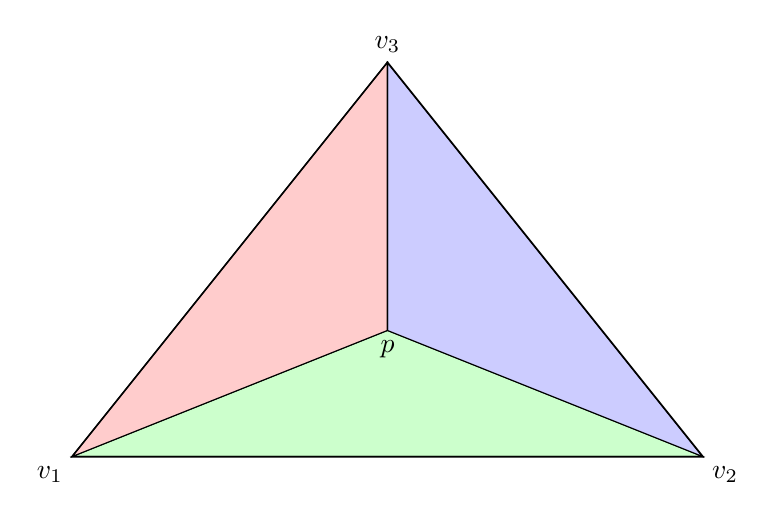
\begin{tikzpicture}
    \coordinate (L1) at (0,0);
    \coordinate (L2) at (8,0);
    \coordinate (L3) at (4,5);
    \coordinate (X) at (4,1.6);

    \draw[thick] (L1) -- coordinate[midway](md3) (L2)
                      -- coordinate[midway](md1) (L3)
                      -- coordinate[midway](md2) (L1) -- cycle;
    \filldraw[draw=black, fill=green!20] (L1) -- (X) -- (L2) -- cycle;
    \filldraw[draw=black, fill=red!20] (L1) -- (X) -- (L3) -- cycle;
    \filldraw[draw=black, fill=blue!20] (L3) -- (X) -- (L2) -- cycle;
    \draw (L1) node [below left] {$v_1$}
       -- (L2) node [below right] {$v_2$}
       -- (L3) node [above] {$v_3$}
       -- (X) node [below] {$p$};
    \end{tikzpicture}
    \\
    Let call the red area $w_1$, the blue green one $w_2$ and the blue one $w_3$. Normalazing each of them by the area of the triangle, we will get three values ($\lambda_1, \lambda_2, \lambda_3$) that are the barycentric coordinates of $p$ with respect to the triangle [$v_1, v_2, v_3$].
\\ \\ WRITE!!!!!!! introduction and all properties

\section{Linear Interpolation}
The standard linear interpolated visualisation is made passing three attributes (colors) for each vertex of a triangle. OpenGL will interpolate linearly the colors. That is possible thanks to the barycentric coordinates that will tell how much of each color is being mixed at any position.

\section{Flat Shading}

\section{Gouraud Shading}

\section{Gaussian Curvature}
\textit{Gaussian Curvature} works like a logical \texttt{AND}, it will check if there is a curvature along both directions.

\begin{figure}[h]
  \minipage[b]{.6\linewidth}
  \centering
  \scalebox{0.7}{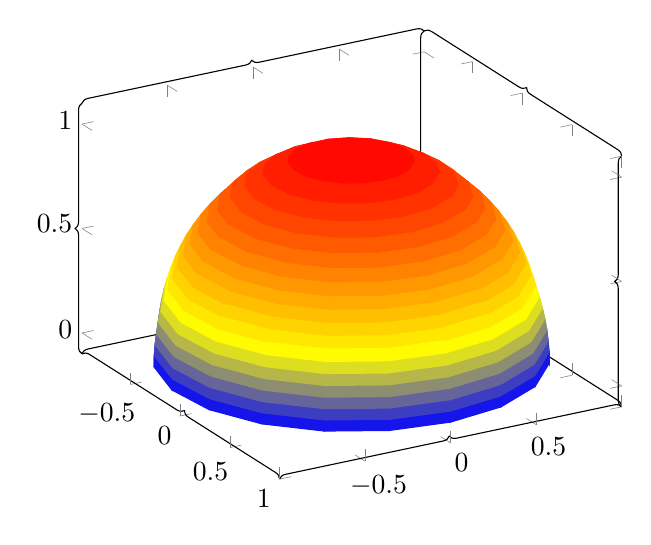
\begin{tikzpicture}
  \begin{axis}[view={60}{30}]
      \addplot3[surf,shader=flat,
          samples=20,
          domain=1:0,y domain=0:2*pi,
          z buffer=sort]
          ({sqrt(1-x^2) * cos(deg(y))},
       {sqrt( 1-x^2 ) * sin(deg(y))},
       x);
  \end{axis}
  \end{tikzpicture}}
  \caption{Positive gaussian curvature}\label{fig:positive-gaussian}
  \endminipage
  \minipage[b]{.6\linewidth}
  \centering
  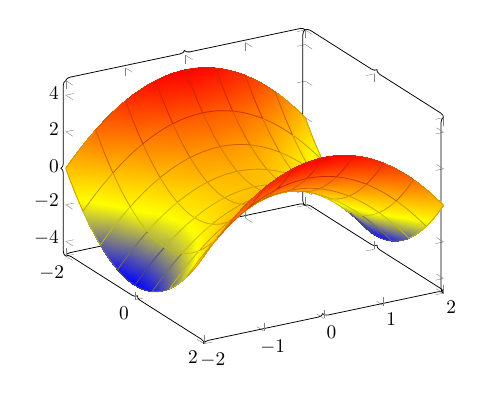
\begin{tikzpicture}[scale=0.7]
    \begin{axis}[view={60}{30}]
    \addplot3[patch,patch refines=3,
    shader=faceted interp,
    patch type=biquadratic]
    table[z expr=x^2-y^2]
    {
        x  y
        -2 -2
        2  -2
        2  2
        -2 2
        0  -2
        2  0
        0  2
        -2 0
        0  0
    };
  \end{axis}
  \end{tikzpicture}
  \caption{Negative gaussian curvature}\label{fig:negative-gaussian}
  \endminipage
\end{figure}

\chapter{GPU program}
A program that runs on GPU is called \textit{shader}. Shaders are principally used to modify the representation and the behaviour of 3D objects. They are also used to create lighting effects. Shaders can perform tasks efficiently thanks to the GPU. That guarantees faster results than CPU since GPU is designed to work in parallel.

\subsection{GPU pipeline}
A program allows us to control the rendering pipeline since by default there is no pipeline set in OpenGL. It takes a set of vertices as input, then the \textit{vertex shader} transforms them (translation, rotation, projection...) and passes the transformed vertices to the \textit{geometry shader}. This shader takes vertices to create primitive shapes and then it rasterizes them. These rasterized flat images are then passed as input to the \textit{fragment shader} that adds the lighting, apply textures and color these images (Fig. \ref{fig:gpu-pipeline}).

\begin{figure}[!h]
    \centering
    \scalebox{0.85}{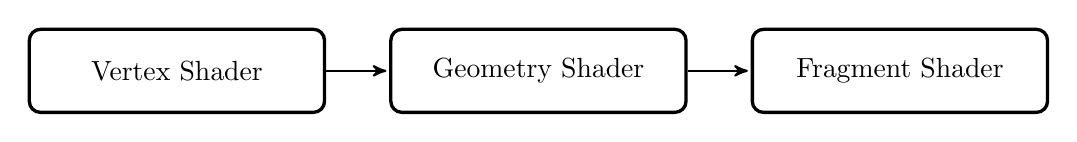
\begin{tikzpicture}
        [node distance=.8cm,
        start chain=going right,]
        \node[punktchain, join] (vs) {Vertex Shader};
        \node[punktchain, join] (gs)  {Geometry Shader};
        \node[punktchain, join] (fs)  {Fragment Shader};
    \end{tikzpicture}}
    \scalebox{0.9}{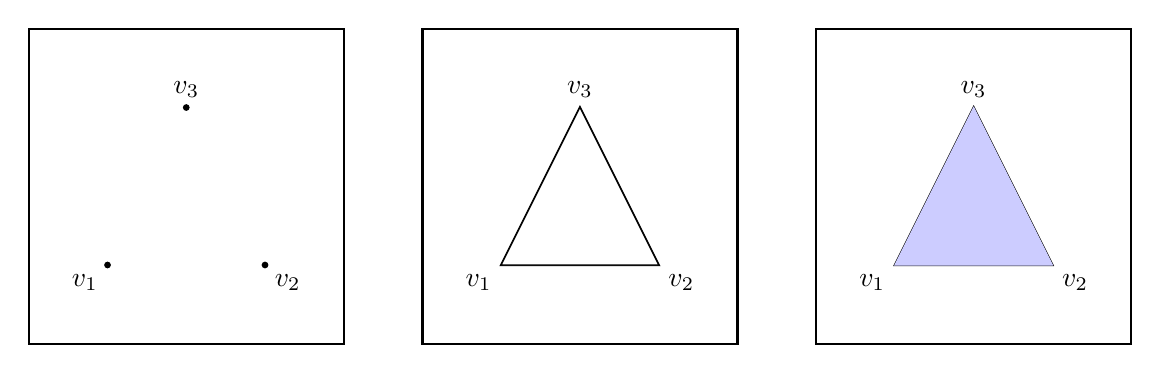
\begin{tikzpicture}
        \coordinate (L1) at (6,0);
        \coordinate (L2) at (8,0);
        \coordinate (L3) at (7,2);

        \coordinate (S1) at (5,-1);
        \coordinate (S2) at (9,-1);
        \coordinate (S3) at (5,3);
        \coordinate (S4) at (9,3);

        \draw[thick] (S1) --  (S2)
                        --  (S4)
                        --  (S3)
                        --  (S1) -- cycle;


        \coordinate (L11) at (11,0);
        \coordinate (L12) at (13,0);
        \coordinate (L13) at (12,2);

        \coordinate (S11) at (10,-1);
        \coordinate (S12) at (14,-1);
        \coordinate (S13) at (10,3);
        \coordinate (S14) at (14,3);


        \draw[thick] (L11) -- (L12)
                        -- (L13)
                        -- (L11) -- cycle;

        \draw[thick] (S11) --  (S12)
                        --  (S14)
                        --  (S13)
                        --  (S11) -- cycle;

        %%%
        \coordinate (L21) at (16,0);
        \coordinate (L22) at (18,0);
        \coordinate (L23) at (17,2);

        \coordinate (S21) at (15,-1);
        \coordinate (S22) at (19,-1);
        \coordinate (S23) at (15,3);
        \coordinate (S24) at (19,3);


        \draw[thick] (L21) -- (L22)
                        -- (L23)
                        -- (L21) -- cycle;

        \draw[thick] (S21) --  (S22)
                        --  (S24)
                        --  (S23)
                        --  (S21) -- cycle;
        \filldraw[draw=black, fill=white] (L11) -- (L12) -- (L13) -- cycle;
        \filldraw[draw=blue!20, fill=blue!20] (L21) -- (L22) -- (L23) -- cycle;
        \draw (L1) node [below left] {$v_1$}
            (L2) node [below right] {$v_2$}
            (L3) node [above] {$v_3$};
        \filldraw (6,0) circle (1pt);
        \filldraw (8,0) circle (1pt);
        \filldraw (7,2) circle (1pt);

        \draw (L11) node [below left] {$v_1$}
            (L12) node [below right] {$v_2$}
            (L13) node [above] {$v_3$};

        \draw (L21) node [below left] {$v_1$}
            (L22) node [below right] {$v_2$}
            (L23) node [above] {$v_3$};
    \end{tikzpicture}}
    \caption{GPU pipeline \cite{WEBSITE:shadertutorial}} \label{fig:gpu-pipeline}
\end{figure}

\subsection{Vertex Shader}
The program that performs vertex operations is called \textit{vertex shader}. It receives one vertex at a time and then it passes the output to a \textit{fragment shader} or to a \textit{geometry shader}, if any.

\subsection{Fragment Shader}
\textit{Fragment shader} performs color computation for every visible pixel of the rasterized object. It works on a fragment at a time, but thanks to the power of GPU it can work in parallel for all vertices (\textit{vertex shader}) and fragments (\textit{fragment shader}).

\subsection{Geometry Shader}
\textit{Geometry shader} is used for layered rendering. It takes as input a set of vertices (single primitive, example: triangle or a point) and it transforms them before sending to the next shader stage. In this way, we can obtain different primitives.
Each time we call the function \texttt{EmitVertex()} the vector currently set to \texttt{gl\_Position} is added to the primitive. All emitted vertices are combined for the primitive and output when we call the function \texttt{EndPrimitive()}.
\cite{WEBSITE:learnopengl}


\chapter{Vertex area based}
\label{section:vertex-area-chapter}
The first goal is to extend the idea of flat shading from triangles to vertices and edges. The idea of flat shading is to draw all the pixels of a triangle with the same colour, and as such it is a natural way to visualize data given at the triangles (for example, the colour of an object, resulting from the lighting calculation using the triangle normal). The extension of this approach is to split the surface of the triangle mesh likewise into regions around vertices and edges and draw all pixels in these regions with the same colour, thus visualizing data given at the vertices or edges of the mesh in a piecewise constant, not necessarily continuous way, resembling the classical triangle flat shading. The aforementioned regions can easily be defined using barycentric coordinates and a simple GPU fragment program can be used to find out for each pixel to which region is belongs and which colour it should be painted with. Examples of vertex and edge data include discrete Gaussian and discrete mean value curvature. The results of this new technique should then be compared to the standard approach mentioned in the beginning.



%%%%%%%%%%%%%

\subsection{Region around a vertex}
We can split the surface of triangle meshes into regions around vertex (Fig. \ref{fig:vertex-area}) and color them.
These regions can be determined using barycentric coordinates and GPU fragment program. Visualizing data given at the vertices or edges of the mesh in a piecewise constant simulates the classical triangle flat shading.
An example of this vertex data is the discrete Gaussian curvature.
\begin{figure}[h]
    \centering
    \minipage[b]{.4\linewidth}
    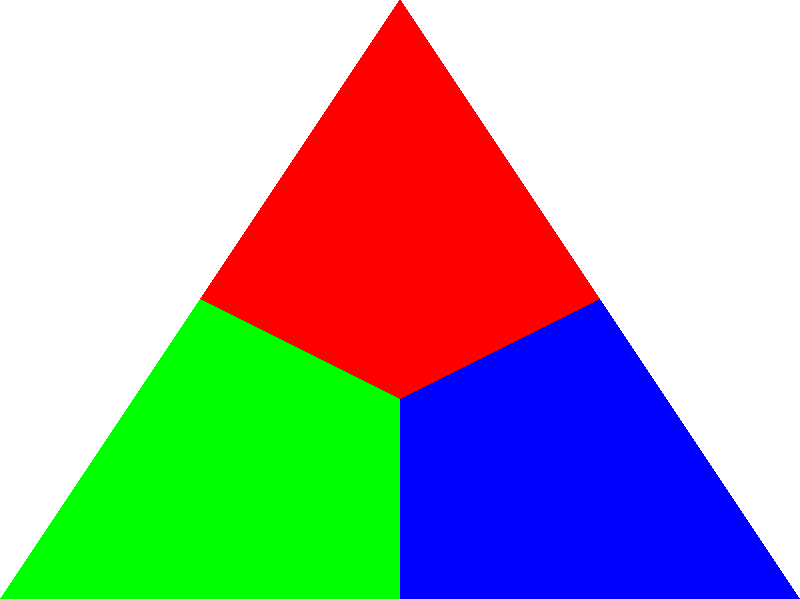
\includegraphics[scale=0.15]{images/max.png}
    \caption{Vertex based area}\label{fig:max-diagram}
    \endminipage\hfill
    \minipage[b]{.4\linewidth}
    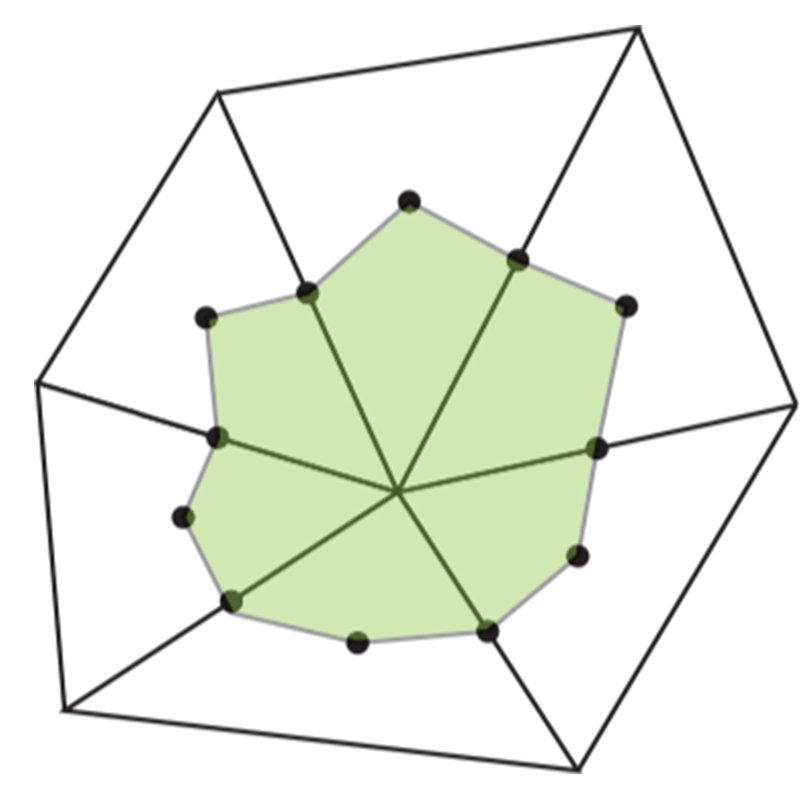
\includegraphics[scale=0.15]{images/vertex-area.png}
    \caption{Region around a vertex}\label{fig:vertex-area}
    \endminipage
\end{figure}

%%%%%%%%%%%%%

\subsubsection{Max diagram - Vertex based area} \label{section:max-diagram}
Passing barycentric coordinates to the \textit{fragment shader} will clearly demonstrate that we can get results different from the classic color interpolation.
%https://www.redblobgames.com/x/1730-terrain-shader-experiments/
\cite{WEBSITE:1}
%----------
There are different approaches to color interpolation focusing on the distance from vertices. For each point in a triangle, we can easily determine its closest vertex, which we use as a cue for coloring.
A different approach from interpolating, can be found coloring vertex areas based on the minimum barycentric coordinate.
The color is given by the region farthest from a vertex (Fig. \ref{fig:max-diagram}, Pseudocode \ref{appendix:max-diagram}).

%%%%%%%%%%%%%

\subsection{Flat shading extension} \label{section:extend-flat-shading-lighting}
An extension of \textit{flat shading} would be to have each vertex area to be in one constant color. This color can be taken from shading interpolation using the normal at the vertex and the vertex position.
The color will then be computed as in \textit{Gouraud shading}.
The idea is to compute the color per vertex but instead of linearly interpolated it in each triangle (as \textit{Gouraud shading} does) we color regions around a vertex with that constant color.
To implement it, the barycentric coordinates, the vertex color, the normal at the vertex and the lighting calculations must be passed to the \textit{fragment shader}.
We want to avoid an automatic interpolation of colors, in order to return the resulting color using the \textit{max diagram} we have used a \textit{Geometry shader} that have access to all three vertex colors in \textit{fragment shader}. (Pseudocodes: \ref{appendix:vs-flat-shading-lighting}, \ref{appendix:gs-flat-shading-lighting}, \ref{appendix:fs-flat-shading-lighting})

\subsubsection{Comparison}
Gouraud shading vs extension flat shading.
TODO

%%%
\subsection{Discrete Gaussian Curvature}
\label{section:vertex-area-gaussian-curvature}
Another interesting alternative data visualization technique is to compute the \textit{Gaussian curvature} per vertex. That can be done summing up, for each vertex, angles at this vertex with adjacent triangles and then subtracting this value to $2\pi$.
After having obtain this value, called \textit{angle defect} (Fig. \ref{fig:gc-angle}), we map linearly this value to a color range.
The resulting color will be the vertex flat shading visualisation of \textit{Gaussian curvature}.
$$K(V) = 2\pi - \sum_j \theta_j$$
%%
\begin{figure}[!h]
    \centering
    \begin{tikzpicture}
        \coordinate (J) at (3.1,2.9);
        \coordinate (circle) at (3.1,2.9);
        \node[anchor=south west,inner sep=0] at (0,0) {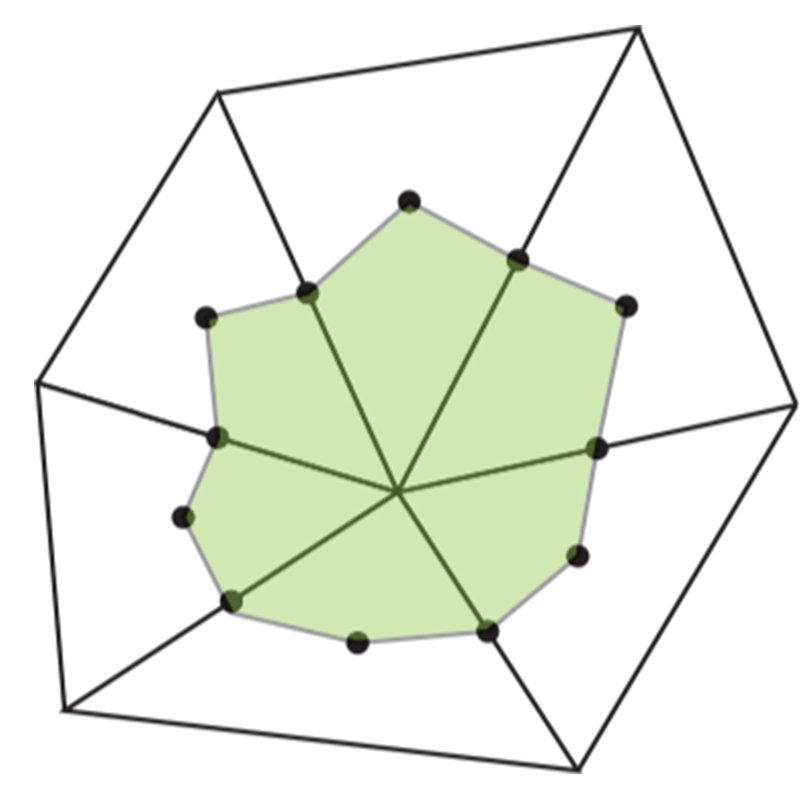
\includegraphics[scale=0.2]{images/vertex-area.png}};
        \draw (J) node [below left] {$j$};
        \filldraw (2.8, 2.2) circle (2pt);
        \begin{scope}[line width=0.4mm, line cap=round]
            \draw (3.2,1.7) arc (295:360:0.7cm) node[near start,right] {$\theta_j$};
        \end{scope}
    \end{tikzpicture}
    \caption{Angle defect}\label{fig:gc-angle}
\end{figure}
%%
\textit{Gaussian curvature} returns a constant color around each vertex (Fig. \ref{fig:gc-icosahedron}, Pseudocode \ref{appendix:vs-gaussiancurvature}).
\begin{figure}[h]
    \centering
    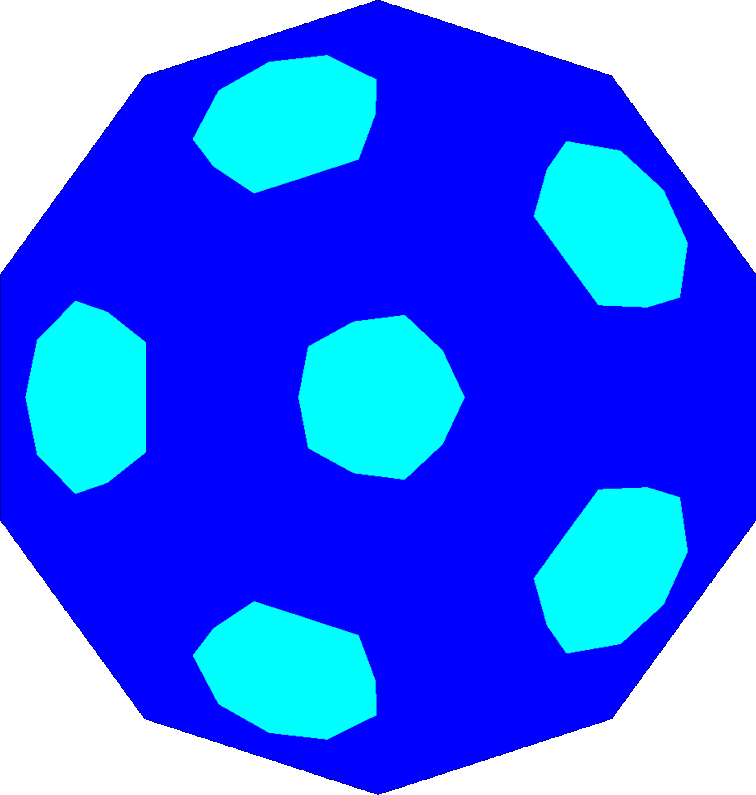
\includegraphics[scale=0.2]{images/gaussian-ball.png}
    \caption{Gaussian curvature on icosahedron}\label{fig:gc-icosahedron}
\end{figure}
TODO: update image 3.4
%%%%%%%%

\subsection{Interpolated Gaussian Curvature}
aka Gouraud Shading Gaussian Curvature
TODO

\subsubsection{Comparison}
We want now to compare the \textit{Gaussian curvature} (Fig. \ref{fig:gaussian-interpolated-horse}) with the \textit{interpolated Gaussian curvature}. In Fig. \ref{fig:gaussian-horse} each vertex area is colored applying the method \textit{max diagram} described in the above subsection \ref{section:max-diagram}. Instead, in Fig. \ref{fig:gaussian-interpolated-horse} the color is obtained with a linear interpolation.
\begin{figure}[!htb]
\centering
  \minipage{0.4\textwidth}
    % \includegraphics[width=\linewidth]{images/}
    \caption{Interpolated Gaussian curvature} \label{fig:gaussian-interpolated-horse}
  \endminipage\hfill
  \centering
  \minipage{0.4\textwidth}%
    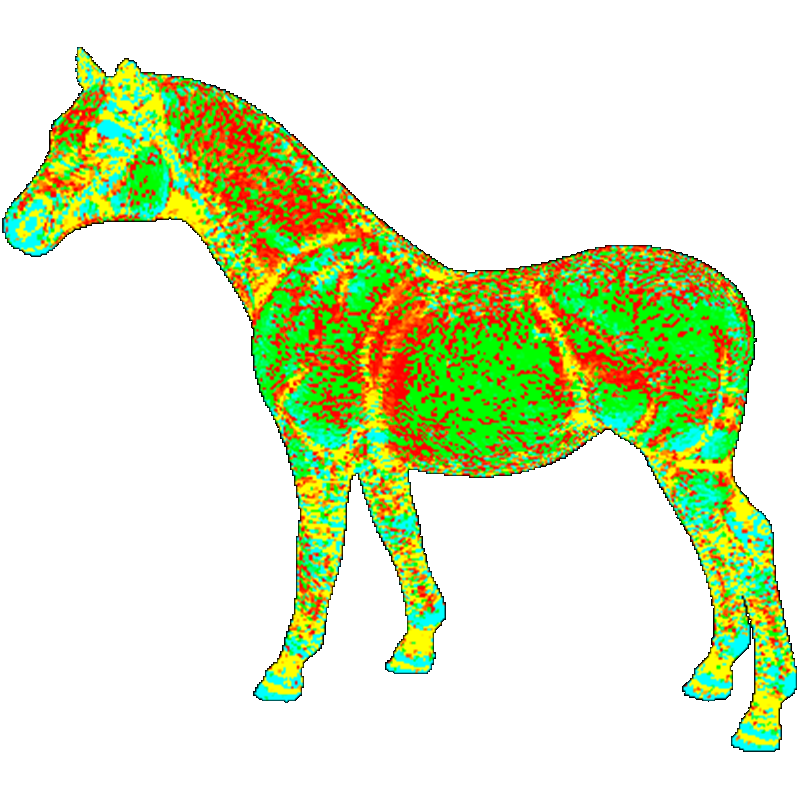
\includegraphics[width=\linewidth]{images/gaussian-horse.png}
    \caption{Gaussian curvature}\label{fig:gaussian-horse}
  \endminipage
  \end{figure}

Visualization of the principal curvatures of the model as colors from blue (highest values of curvature) to red (lower values of curvature), in both Fig. \ref{fig:gaussian-horse} and Fig. \ref{fig:gaussian-interpolated-horse}, better highlighs the geometry of the horse.
These changes of curvature, positive (blue), flat (green) and negative regions (red), better emphasises the 3-dimensionality of the model.
TODO
% \textit{Gaussian curvature} better shows the muscle constrasts given a more realistic character to the horse than the model obtained using the \textit{interpolated Gaussian curvature}.


% \subsection{Min diagram - Edge based area}
% A different approach from interpolating, can be found coloring edge areas based on the minimum barycentric coordinate.
% The color is given by the region closest to the vertex.

% \chapter{Conclusion}
% Making computation per vertex (e.g. \textit{Flat Shading}) is more efficient because in general, a model has fewer vertices than triangles as shown in table \ref{table:model-table-vertices}.
For example, the armadillo model has $15002$ vertices and $30000$ triangles, then make calculation per vertex instead of triangle results in half of the computations.

\begin{table}[!h]
    \centering
\begin{tabular}{l*{6}{c}r}
    \centering
    Model              & \#vertices & \#triangles & Improvement\\
    \hline
    Armadillo          & 15002 & 30000 & 49\%\\
    Eight              & 766 & 1536 & 50\% \\
    Genus3             & 6652 & 13312 & 50\% \\
    Horse              & 48485 &  96966 & 49\%\\
    Icosahedron\_1      &  42 & 80 & 47\%\\
    Icosahedron\_2      &  162 & 320 & 49\% \\
    Icosahedron\_3      & 642 &  1280 & 50\%
\end{tabular}
\caption{Number of vertices and triangles in models. Making computations per vertex result in an efficiency improvement of $\approx$ 50\%.}
\label{table:model-table-vertices}
\end{table}

Making computation per edge would also be more efficient, because edges are shared between $2$ triangles in a mesh.

\subsection{Application Software}
I have developed an application for alternative data visualization using the power of barycentric coordinates and GPU programming.
\begin{figure}[!h]
    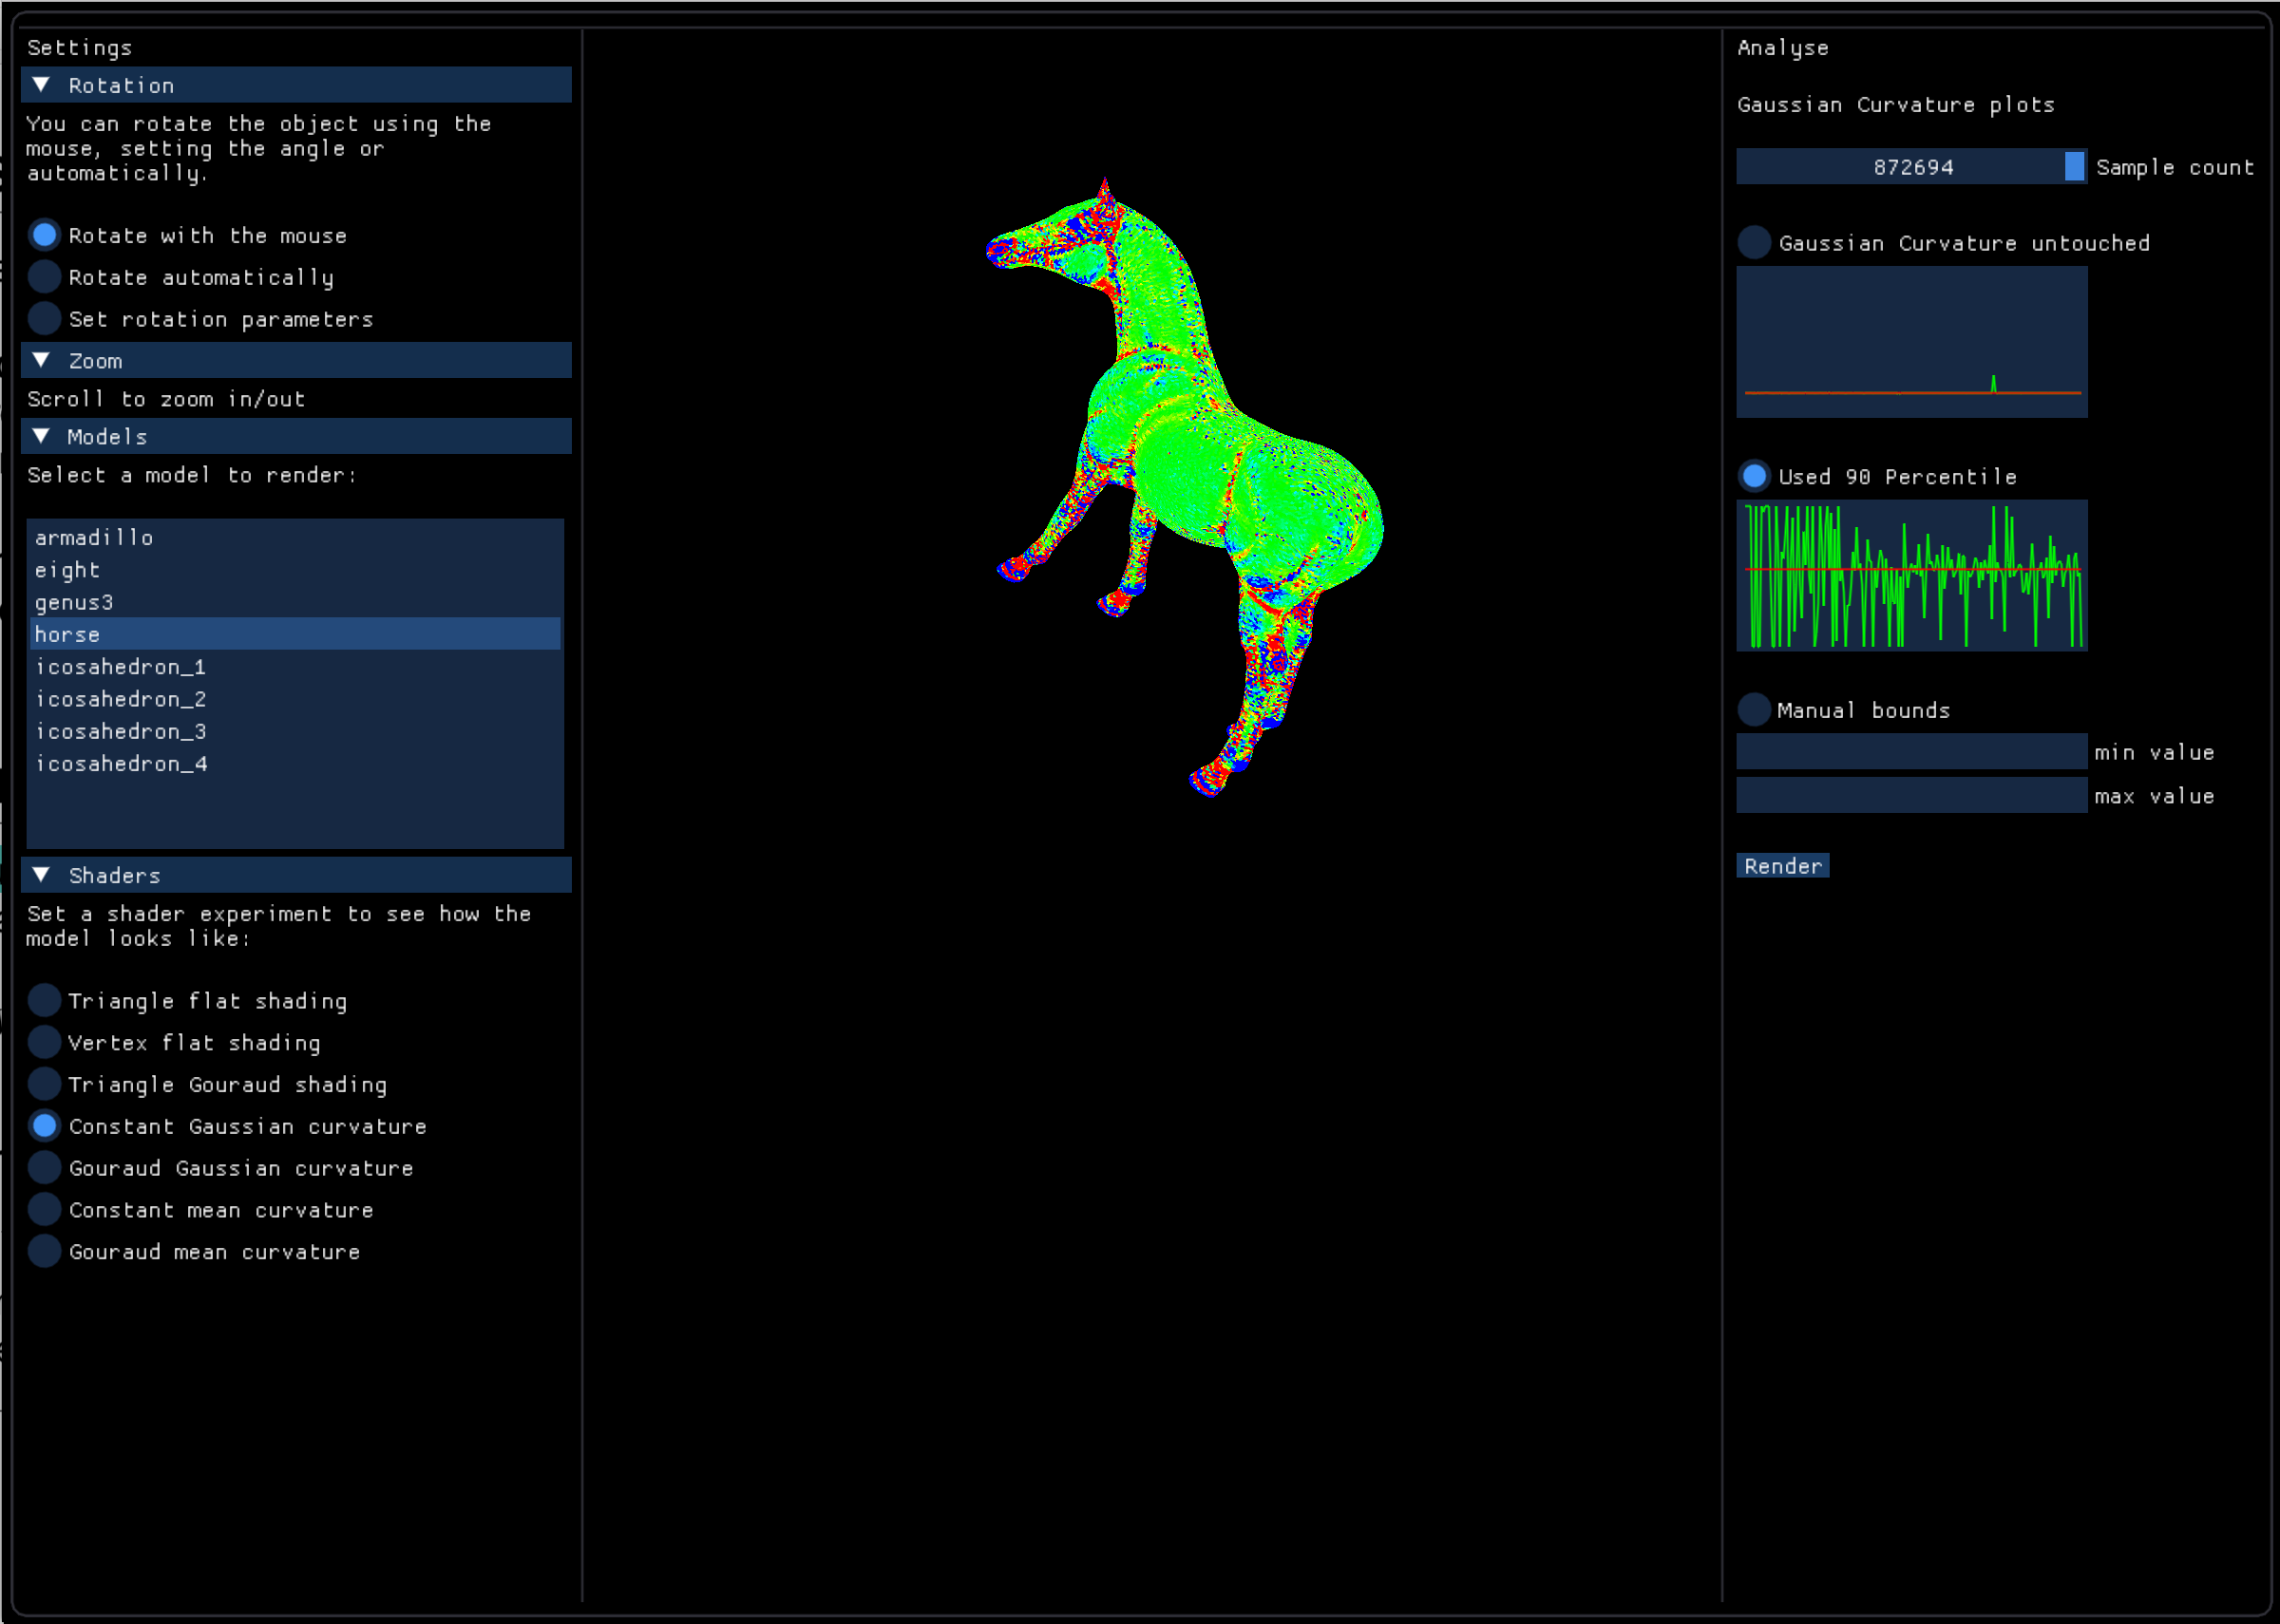
\includegraphics[scale=0.4]{images/program.png}
    \caption{Software}
    \label{fig:software}
\end{figure}
This application allows the user to upload different models, choose different shaders, zoom or rotate the model.
In Fig. \ref{fig:software}, a \textit{constant Gaussian curvature} shader is chosen for a model using a $90 \; percentile$, on the right graphs plot Gaussian curvature values obtained for each vertex. The first graph shows the real values of Gaussian curvature without removing the outliers. The second graph shows just the values in the $90 \; percentile$ (all the outliers were discarded).

\subsection{Architecture}
The application was developed in c++, for the real-time graphics programming (e.g. create the scene viewer, enabling the manipulation of 3D scenes) I have used OpenGL $3.3$ and GLSL.

As graphical user interface I have used a library called \textit{Dear ImGui}. This library has no external dependencies and it is designed to create content creation tools and visualization/debug tools. It is suited to integration in games engine (for tooling), real-time 3D applications or any applications on console platforms where operating system features are non-standard.

To allow the creation of an OpenGL context, the definition of window parameters and to handle user inputs I have used the \textit{GLFW3} library.

Since there are different versions of OpenGL drivers, to retrieve the location of the functions required and to store them in function pointers for later use, I have used \textit{GLAD} library that loads all relevant OpenGL functions according to that version at compile-time.

\subsection{Comparison with meshlab}
All the values obtained for the \textit{Gouraud Gaussian curvature} and \textit{Gouraud mean curvature} were compared to the results provided by the program \textit{meshlab}\footnote{Meshlab is an open source system for processing and editing 3D triangular meshes.
It provides a set of tools for editing, cleaning, healing, inspecting, rendering, texturing and converting meshes. It offers features for processing raw data produced by 3D digitization tools/devices and for preparing models for 3D printing. \url{http://www.meshlab.net/}}.


\begin{table}[!h]%gauss
    \centering
\begin{tabular}{l*{6}{c}r}
    \centering
    Model              & our software &  meshlab   & absolute difference\\
    \hline
    Armadillo          & [-33034.20, 90017.90] & [-33033.84, 90019.63] & [0.36, 1.73] \\
    Eight              & [-116.89, 58.33] & [-116.89, 58.33] & [0.00, 0.00] \\
    Genus3             & [-1753.20, 209.18] & [-1753.20, 209.18] & [0.00, 0.00]  \\
    Horse              & [-321731, 1930410] &  [-4177.14, 4853.23] & [317553.86 1925556.77]\\
    Icosahedron\_1      &  [1.07, 1.08] & [1.07, 1.08] & [0.00, 0.00] \\
    Icosahedron\_2      &  [1.01, 1.02] & [1.01, 1.02] & [0.00, 0.00] \\
    Icosahedron\_3      & [1.00, 1.00] &  [1.00, 1.00] & [0.00, 0.00]
\end{tabular}
\caption{Our Gouraud Gaussian curvature values ([min, max]) and meshlab Gouraud Gaussian curvature values ([min, max]).}
\label{table:table-gaussian-meshlab}
\end{table}



\begin{table}[!h]%mean
    \centering
\begin{tabular}{l*{6}{c}r}
    \centering
    Model              & our software &  meshlab  & absolute difference\\
    \hline
    Armadillo          & [-289.74, 392.54] & [-289.74, 392.54] & [0.00, 0.00]\\
    Eight              & [1.35, 10.96] & [1.35, 10.96] & [0.00, 0.00]\\
    Genus3             & [-7.02, 117.34] & [-7.03, 117.34] & [0.00, 0.00] \\
    Horse              & [-500.96, 1202.51] &  [-500.96, 1202.51] & [0.00, 0.00]\\
    Icosahedron\_1      &  [0.10, 1.00] & [0.10, 1.00] & [0.00, 0.00]\\
    Icosahedron\_2      &  [0.10, 1.00] & [0.10, 1.00]& [0.00, 0.00] \\
    Icosahedron\_3      & [0.10, 1.00] &  [0.10, 1.00] & [0.00, 0.00]
\end{tabular}
\caption{Our Gouraud mean curvature values ([min, max]) and meshlab Gouraud mean curvature values ([min, max]).}
\label{table:table-mean-meshlab}
\end{table}



% See~\cite{DUMMY:1}.
% \printbibliography
% \bibliography{report}

% \cite{BOOK:1}

\bibliography{report}
\bibliographystyle{plain}


% \begin{thebibliography}{9}
%   % \bibitem{ddd}
%   % Michel Goossens, Frank Mittelbach, and Alexander Samarin.
%   % \textit{The \LaTeX\ Companion}.
%   % Addison-Wesley, Reading, Massachusetts, 1993.

%   % \bibitem{einstein}
%   % Albert Einstein.
%   % \textit{Zur Elektrodynamik bewegter K{\"o}rper}. (German)
%   % [\textit{On the electrodynamics of moving bodies}].
%   % Annalen der Physik, 322(10):891–921, 1905.
%   \bibitem{barycenterCutKnot}
%   \textit{Cut-the-knot}, Alexander Bogomolny.
%   \\\texttt{www.cut-the-knot.org}
% \end{thebibliography}


\appendix
\chapter{Pseudocodes}
\begin{lstlisting}[caption={Max diagram - Vertex area (Section: \ref{section:max-diagram})\label{appendix:max-diagram}}]
    #version 330 core

    in vec3 coords;
    in vec4 wedge_color[3]; // an array of 3 vectors of size 4 (since it is a triangle)
    out vec4 fragColor;

    void main()
    {
            if (coords[0] > coords[1]) {
                if (coords[0] > coords[2]) { // 0 > 1 && 0 > 2
                    fragColor = wedge_color[0];
                }
                else { // 0 > 1 && 2 > 0 --> 2 > 0 > 1
                    fragColor = wedge_color[2];
                }
            }
            else {
                if (coords[1] > coords[2]) { // 1 > 0 && 1 > 2
                    fragColor = wedge_color[1];
                }
                else { // 1 > 0 && 1 < 2 --> 2 > 1 > 0
                    fragColor = wedge_color[2];
                }
            }
    }
\end{lstlisting}

\vspace{10pt}

\begin{lstlisting}[caption={Min diagram - Edge area (Section: \ref{section:min-diagram})\label{appendix:min-diagram}}]
    #version 330 core
    in vec3 coords;
    in vec4 wedge_color[3]; // an array of 3 vectors of size 4 (since it is a triangle)
    out vec4 fragColor;

    void main()
    {
        if (coords[0] < coords[1]) {
            if (coords[0] < coords[2]) {
                fragColor = wedge_color[0];
            }
            else {
                fragColor = wedge_color[2];
            }
        }
        else {
            if (coords[1] < coords[2]) {
                fragColor = wedge_color[1];
            }
            else {
                fragColor = wedge_color[2];
            }
        }
    }
\end{lstlisting}
\vspace{10pt}

\begin{lstlisting}[caption={Edge structure} (Section \ref{section:edge-struct})]
    struct edge
    {
        float norm_edge;
        int index_v1;
        int index_v2;
        Point3d n1;
        Point3d n2;
        float value_mean_curvature;
        float cot_alpha;
        float cot_beta;
        float area_t1;
        float area_t2;
    };
\end{lstlisting} \label{Pseudocode:edge}

\vspace{10pt}

\begin{lstlisting}[caption={Region $\mathcal{A}_{Mixed}$ on an arbitrary mesh. \cite{meshlab} (Section: \ref{section:localaveraging})\label{appendix:localaveraging}}]
    A_Mixed = 0
    For each triangle T from the 1-ring neighborhood of x
    If T is non-obtuse (Voronoi safe)
        A_Mixed += Voronoi region of x in T
    Else
        If x is obtuse
            A_Mixed += area(T)/2
        Else
            A_Mixed += area(T)/4
    \end{lstlisting}

\vspace{10pt}

\begin{lstlisting}[caption={Vertex Shader for vertex/triangle flat shading and triangle Gouraud shading using lighting (Section: \ref{section:extend-flat-shading-lighting})\label{appendix:vs-flat-shading-lighting}}]
    #version 330 core
    layout (location = 0) in vec3 aPos;
    layout (location = 1) in vec3 aNormal;
    layout (location = 5) in vec3 aNormalTriangle;

    struct Light {
        vec3 position;

        vec3 ambient;
        vec3 diffuse;
        vec3 specular;
    };

    out vec4 color;

    uniform mat4 model;
    uniform mat4 view;
    uniform mat4 projection;

    uniform vec3 view_position;
    uniform Light light;
    uniform float shininess;

    uniform bool isFlat;


    // get specular color at current Pos
    vec3 get_specular(vec3 pos, vec3 normal, vec3 light_direction) {

        // get directional vector to the camera from pos
        vec3 view_direction = normalize(view_position - pos);

        // specular shading
        vec3 reflect_direction = - normalize(reflect(light_direction, normal));
        float specular_intensity = pow(max(dot(reflect_direction, view_direction), 0.0), shininess);

        // get resulting color
        return light.specular * specular_intensity;
    }


    // return diffuse at current Pos
    vec3 get_diffuse(float lambert_term) {
        return light.diffuse * lambert_term;
    }

    vec4 get_result_color_lighting(vec3 pos, vec3 normal, vec3 light_position) {
        vec3 light_direction = normalize(light_position - pos);
        float diffuse_intensity = max(dot(light_direction, normal), 0.0);

        vec3 ambient = light.ambient;
        vec3 diffuse = get_diffuse(diffuse_intensity);

        if(diffuse_intensity > 0.0001){
            vec3 specular = get_specular(pos, normal, light_direction);
            return vec4((ambient + diffuse + specular), 1.0);
        }

        return vec4((ambient + diffuse) , 1.0);
    }


    void main() {

        vec3 world_position = vec3(model * vec4(aPos, 1.0));
        vec3 world_normal;

        if(isFlat){ // triangle normal
            world_normal = mat3(transpose(inverse(model))) * aNormalTriangle;
        } else { // vertex normal
            world_normal = mat3(transpose(inverse(model))) * aNormal;
        }

        vec3 light_pos = vec3(projection * vec4(light.position, 1.0));

        color = get_result_color_lighting(world_position, world_normal, light_pos); // color obtained with lighting calculations

        gl_Position = projection * view * model * vec4(aPos, 1.0);
    }


\end{lstlisting}

\vspace{10pt}

\begin{lstlisting}[caption={Vertex Shader for constant/Gouraud Gaussian curvature and constant/Gouraud mean curvature (Sections: \ref{section:gc-curvature} and \ref{section:mc-curvature})}]
    #version 330 core
    layout (location = 0) in vec3 aPos;
    layout (location = 2) in vec3 gaussian_curvature;
    layout (location = 3) in vec3 mean_curvature_edge;
    layout (location = 4) in vec3 mean_curvature_vertex;

    out vec4 color;

    uniform mat4 model;
    uniform mat4 view;
    uniform mat4 projection;

    uniform float min_curvature;
    uniform float max_curvature;

    uniform bool isGaussian;
    uniform bool isMeanCurvatureEdge;

    vec3 interpolation(vec3 v0, vec3 v1, float t) {
        return (1 - t) * v0 + t * v1;
    }

    vec3 hsv2rgb(vec3 c)
    {
        vec4 K = vec4(1.0, 2.0 / 3.0, 1.0 / 3.0, 3.0);
        vec3 p = abs(fract(c.xxx + K.xyz) * 6.0 - K.www);
        return c.z * mix(K.xxx, clamp(p - K.xxx, 0.0, 1.0), c.y);
    }


    vec4 get_result_color(){
        float val = gaussian_curvature[0]; // gaussian_curvature is a vec3 composed by same value
        if(!isGaussian && !isMeanCurvatureEdge){
            val = mean_curvature_vertex[0]; // mean curvature is a vec3 composed by same value
        } else if(!isGaussian && isMeanCurvatureEdge){
            val = mean_curvature_edge[0]; // mean curvature is a vec3 composed by same value
        }

        // colors in HSV
       vec3 red = vec3(0.0, 1.0, 1.0); //h s v
       vec3 green = vec3(0.333, 1.0, 1.0);
        vec3 blue = vec3(0.6667, 1.0, 1.0);

        if (val < 0) { //negative numbers until 0
            return vec4(hsv2rgb(interpolation(green, red, min(val/min_curvature, 1.0))), 1.0);
        } else { //from 0 to positive
            return vec4(hsv2rgb(interpolation(green, blue, min(val/max_curvature, 1.0))), 1.0);
        }
    }


    void main() {
        vec3 pos = vec3(model * vec4(aPos, 1.0));

        color = get_result_color();

        gl_Position = projection * view * model * vec4(aPos, 1.0);
    }
\end{lstlisting}

\begin{lstlisting}[caption={Geometry Shader for triangle flat shading, vertex flat shading, constant gaussian curvature, constant mean curvature (Sections: \ref{section:section:vertex-area-chapter} and \ref{section:edge-area-chapter})}]
    #version 330 core

    layout (triangles) in;
    layout (triangle_strip, max_vertices = 3) out;

    in vec4 color[3]; // an array of 3 vectors of size 4 (since it is a triangle)
    out vec3 coords;
    out vec4 wedge_color[3]; // an array of 3 vectors of size 4 (since it is a triangle)

    void main()
    {
        wedge_color[0] = color[0];
        wedge_color[1] = color[1];
        wedge_color[2] = color[2];

        coords = vec3(1.0, 0.0, 0.0);
        gl_Position = gl_in[0].gl_Position;
        EmitVertex();

        coords = vec3(0.0, 1.0, 0.0);
        gl_Position = gl_in[1].gl_Position;
        EmitVertex();

        coords = vec3(0.0, 0.0, 1.0);
        gl_Position = gl_in[2].gl_Position;
        EmitVertex();

        EndPrimitive();
    }
\end{lstlisting}




\end{document}

